\documentclass[12pt, twoside]{article}
\documentclass[12pt, twoside]{article}
\usepackage[letterpaper, margin=1in, headsep=0.2in]{geometry}
\setlength{\headheight}{0.6in}
%\usepackage[english]{babel}
\usepackage[utf8]{inputenc}
\usepackage{microtype}
\usepackage{amsmath}
\usepackage{amssymb}
%\usepackage{amsfonts}
\usepackage{siunitx} %units in math. eg 20\milli\meter
\usepackage{yhmath} % for arcs, overparenth command
\usepackage{tikz} %graphics
\usetikzlibrary{quotes, angles}
\usepackage{graphicx} %consider setting \graphicspath{{images/}}
\usepackage{parskip} %no paragraph indent
\usepackage{enumitem}
\usepackage{multicol}
\usepackage{venndiagram}

\usepackage{fancyhdr}
\pagestyle{fancy}
\fancyhf{}
\renewcommand{\headrulewidth}{0pt} % disable the underline of the header
\raggedbottom
\hfuzz=2mm %suppresses overfull box warnings

\usepackage{hyperref}

\title{IB Mathematics}
\author{Chris Huson}
\date{April 2024} %previously March 2022, 5.6 Exit Note: Compound Interest

\fancyhead[LE]{\thepage}
\fancyhead[RO]{\thepage \\ Name: \hspace{1cm} \,\\}
\fancyhead[LO]{BECA/Huson/Algebra II 4: Exponential functions \& Rational Exponents \\* 3 April 2024}

\begin{document}

\subsubsection*{4.7 PreExam: Exponential Functions and Compound Interest}
I can calculate compound interest \hfill CCSS.HSF.LE.A.2 \\[0.5cm]
$\displaystyle FV=PV \times \left(1+\frac{r}{100k} \right)^{kn}$
where FV is the future value,\\[0.25cm]
PV is the present value, n is the number of years, \\
 k is the number of compounding periods per year, \\
 r\% is the nominal annual rate of interest

\begin{enumerate}
\item Write down the formula for a function $f(x)$ that increases 15\% for each increase of 1 in input value $x$. \vspace{2cm}
\item The price of a share of stock in a particular company is \$2.25 per share in 2010. Assume that it increases in value by 6\% annually thereafter. 
\begin{enumerate}
    \item 	Write an equation representing the value of the stock $P(t)$, in dollars, $t$ years after 2010. \vspace{2cm}
    \item What does $P(30)$ represent in this context? \vspace{2cm}
\end{enumerate}

\item An investment of \$5,000 compounds monthly with an annual interest rate of 4\%.
\begin{enumerate}[itemsep=0.5cm]
    \item How many compounding periods are there per year? \\[0.25cm]
    $k=$
    \item First write the formula for, and then calculate, the account balance of principal and interest after three years.
\end{enumerate} \vspace{2cm}

\newpage
\item The graph shows the exponential function $\displaystyle f(x)$.
\begin{multicols}{2}
    \begin{enumerate}[itemsep=1cm]
        \item Write down the initial value of the function.
        \item By what factor do the values of $f$ increase each time $x$ increases by 1?
        \item By what factor would $f$ increase when the input increases by 10?
    \end{enumerate}
    \begin{center}
    \begin{tikzpicture}[x=1cm, y=0.15cm, xscale=2]
        \draw [thin, color=lightgray, xstep=0.5cm,ystep=0.75cm] (0,0) grid (3,40);
        \draw [thick, ->] (0,0) -- (+3.3,0) node [below]{$x$};
        \draw [thick, ->] (0,0) -- (0,43) node [right]{$y$};        
        \foreach \x in {0,0.5,...,3}
            \draw (\x cm,0) -- (\x cm,0) node[below] {$\x$};
        \foreach \y in {0,10,20,...,40}
            \draw[shift={(0,\y)}] (2pt,0pt)--(-2pt,0pt) node[left]{$\y$};
        \draw [thick, ->, smooth,domain=0.:3.2] plot(\x,{10*(1.5^\x)}) node[below right]{$f$};
        \fill (0,10) ellipse [x radius=1pt, y radius=2pt]  node [below right] {$(0,10)$};
        \fill (1,15) ellipse [x radius=1pt, y radius=2pt] node [below right] {$(1,15)$};
    \end{tikzpicture}
    \end{center}
    \end{multicols}

\item A company depreciates a piece of equipment which was purchased in 2022 at a constant annual rate. The equation representing the value of the equipment $V(t)$, in dollars, $t$ years after 2022 is $\displaystyle V(t)=12,000 \times (0.85)^t$.

\begin{multicols}{2}
    \begin{enumerate}[itemsep=1cm]
        \item Write down the initial value of the equipment.
        \item What does the value 0.85 tell us about the situation?
        \item By what percent does the equipments value decrease each year?
        \item Sketch the graph of the function.
    \end{enumerate}
    \begin{center}
    \begin{tikzpicture}[x=1cm, y=0.004cm, xscale=1]
        \draw [thin, color=lightgray, xstep=1cm,ystep=0.8cm] (0,0) grid (5,1605);
        \draw [thick, ->] (0,0) -- (+5.3,0) node [below]{$t$};
        \draw [thick, ->] (0,0) -- (0,1700) node [right]{$y$};        
        \foreach \x in {0,1,...,5}
            \draw (\x cm,0) -- (\x cm,0) node[below] {$\x$};
        \foreach \y in {0,200,...,1600}
            \draw[shift={(0,\y)}] (2pt,0pt)--(-2pt,0pt) node[left]{$\y$};
        %\draw [thick, ->, smooth,domain=0.:5.2] plot(\x,{1200*(0.85^\x)});
    \end{tikzpicture}
    \end{center}
    \end{multicols}

\end{enumerate}
\end{document}